% D.31 等边△ABC 内一点 P，PA=3、PB=4、PC=5；△APB 绕 A 顺时针旋转 60°
\documentclass[tikz,border=4pt]{standalone}
\usepackage{ctex}
\usepackage{amsmath}
\usetikzlibrary{calc}
\begin{document}
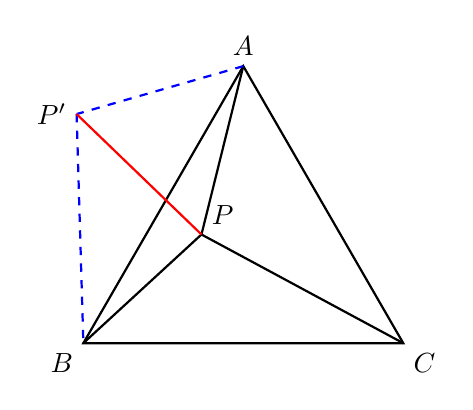
\begin{tikzpicture}[scale=0.6, thick]
  % 等边△：边长 a，使 P 与三边距离合适。取 a≈6.77（费马点经典结果）
  \pgfmathsetmacro{\a}{6.77}
  \coordinate (B) at (0, 0);
  \coordinate (C) at (\a, 0);
  \coordinate (A) at ({\a/2}, {\a*sqrt(3)/2});
  % P 内部：PA=3，PB=4，PC=5；不必精确，目测放置
  \coordinate (P) at (2.5, 2.3);
  % P' = P 绕 A 顺时针旋转 60°
  \coordinate (Pp) at ($(A) + ({cos(-60)*(2.5-\a/2) - sin(-60)*(2.3-\a*sqrt(3)/2)},
                            {sin(-60)*(2.5-\a/2) + cos(-60)*(2.3-\a*sqrt(3)/2)})$);

  \draw (A) -- (B) -- (C) -- cycle;
  \draw (P) -- (A);
  \draw (P) -- (B);
  \draw (P) -- (C);
  \draw[blue, dashed] (A) -- (Pp);
  \draw[blue, dashed] (Pp) -- (B);
  \draw[red] (P) -- (Pp);  % PP'，旋转 60° 后等边连接

  \node[above]       at (A)  {$A$};
  \node[below left]  at (B)  {$B$};
  \node[below right] at (C)  {$C$};
  \node[above right] at (P)  {$P$};
  \node[left]        at (Pp) {$P'$};
\end{tikzpicture}
\end{document}
